
\noindent\begin{minipage}{\textwidth}
    \begin{table}[H]
        \centering
        \caption{Hiperparâmetros e Resultados do Melhor Modelo - swin\_v9\_AM\_opt\_aug}
        \vspace{0.2cm}
        \resizebox{\textwidth}{!}{%
            \begin{tabular}{ll | lrrr}
                \hline
                \multicolumn{2}{c|}{\textbf{Hiperparâmetros}} & \multicolumn{4}{c}{\textbf{Métricas por Classe}} \\ \hline
                \textbf{Parâmetro} & \textbf{Valor} & \textbf{Classe} & \textbf{Precisão} & \textbf{Recall} & \textbf{F1-Score} \\ \hline
    Agendador (\$T\_0\$) & 12 & 31.2 & 0,6302 & 0,5354 & 0,5789 \\ 
Agendador de LR & CosineAnnealingWarmRestarts & 31.3 & 0,4092 & 0,6139 & 0,4911 \\ 
Architecture & swin\_t & 31.4 & 0,5071 & 0,3381 & 0,4057 \\ 
Batch Size & 32 & 32.3 & 0,7099 & 0,4745 & 0,5688 \\ 
Data Augmentation & False & 32.4 & 0,2692 & 0,1207 & 0,1667 \\ 
Decaimento de Peso (WD) & 0,0118 & 33.3 & 0,5077 & 0,5130 & 0,5103 \\ 
Dropout & 0,0059 & 41.4 & 0,2857 & 0,6364 & 0,3944 \\ 
Função de Perda & CrossEntropyLoss & 41.5 & 0,5952 & 0,6410 & 0,6173 \\ 
Hidden Units & 512 & 42.4 & 0,3966 & 0,6765 & 0,5000 \\ 
Label Smoothing & 0,0228 & 44.4 & 0,7273 & 0,5517 & 0,6275 \\ 
\cline{3-6} 
Otimizador & AdamW & \textbf{Média (Macro)} & 0,5038 & 0,5101 & 0,4861 \\ 
Taxa de Aprendizado (LR) & 1,61e-04 & \textbf{MCC} & \multicolumn{3}{c}{0,4249} \\ 
Unfreeze Layers & 2 &  & & &  \\ 
            \hline
            \end{tabular}%
        }
    \end{table}

    \begin{figure}[H]
        \centering
        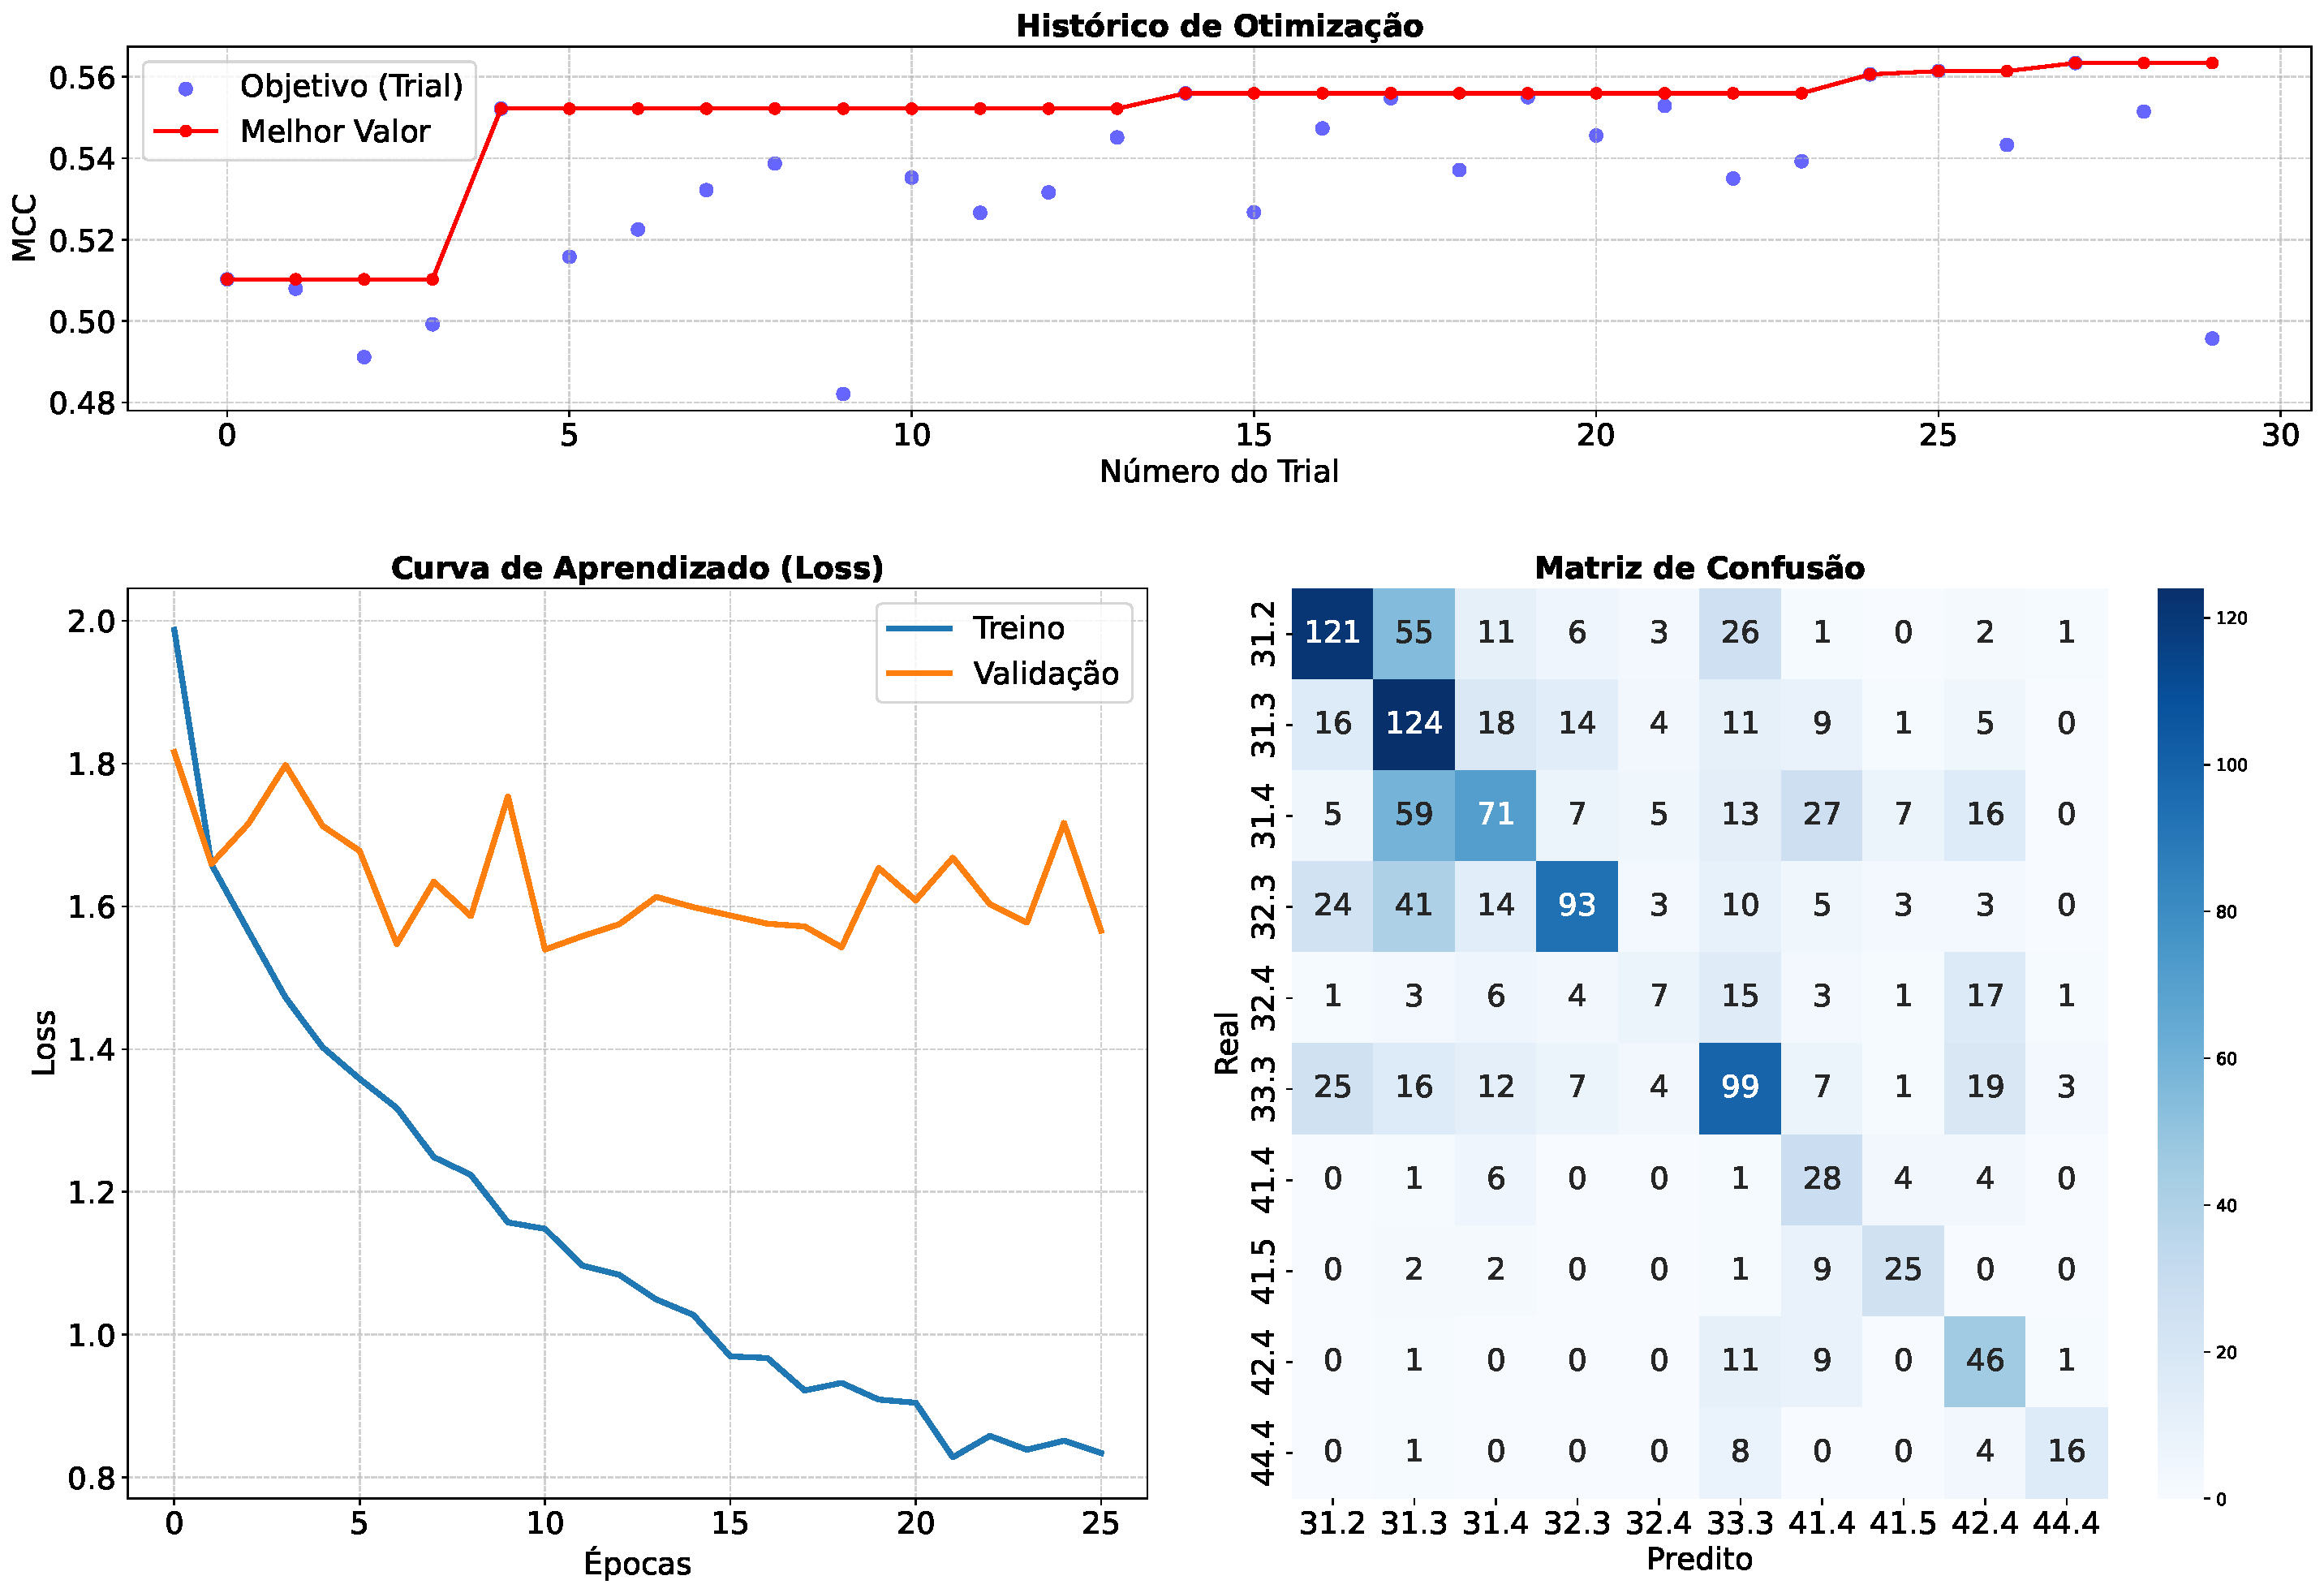
\includegraphics[width=0.85\textwidth]{tex/appendix/experiments/swin_v9_AM_opt_aug/dashboard_consolidado.pdf}
        \caption{Histórico de Otimização, Curvas de Aprendizado e Matriz de Confusão - swin\_v9\_AM\_opt\_aug}
    \end{figure}
\end{minipage}
\clearpage
